% ---------------------------------------------------------------------------
% Codificación Data-Strobe de SpaceWire: sobre el mismo flujo de datos, la línea
% Strobe conmuta únicamente cuando el bit repite al anterior, de modo que entre
% las dos líneas hay exactamente una transición por período de bit. En recepción
% la XOR de ambas devuelve el reloj.
% Fuente del PDF que incluye la memoria (capítulo 2).
%
% La planta es deliberadamente ancha y baja: la figura ilustra un protocolo que
% el lector puede no conocer y tiene que ocupar poco sitio en la página.
%
% Los tres niveles salen de la regla del estándar y son coherentes entre sí:
%   Data  0 1 0 0 1 1 0 1 1 0
%   D     0 1 0 0 1 1 0 1 1 0   (la propia línea de datos)
%   S     0 0 0 1 1 0 0 0 1 1   (conmuta en los bits 3, 5 y 8, los que repiten)
%   CLK   0 1 0 1 0 1 0 1 0 1   (D xor S: un flanco por bit)
%
% Compilar:  pdflatex diagrama_data_strobe.tex
% ---------------------------------------------------------------------------
\documentclass[border=8pt,12pt]{standalone}
\usepackage[utf8]{inputenc}
\usepackage[T1]{fontenc}
\usepackage{lmodern}
\usepackage{tikz}
\usetikzlibrary{arrows.meta, calc}

\definecolor{cPropio}{HTML}{2A78D6}   % azul: las dos líneas del enlace
\definecolor{cIP}{HTML}{EDA100}       % ámbar: el reloj recuperado
\definecolor{cRef}{HTML}{8A8A85}      % gris: rejilla y rótulos
\definecolor{cAcc}{HTML}{C94F4F}      % rojo: las conmutaciones de Strobe

\begin{document}
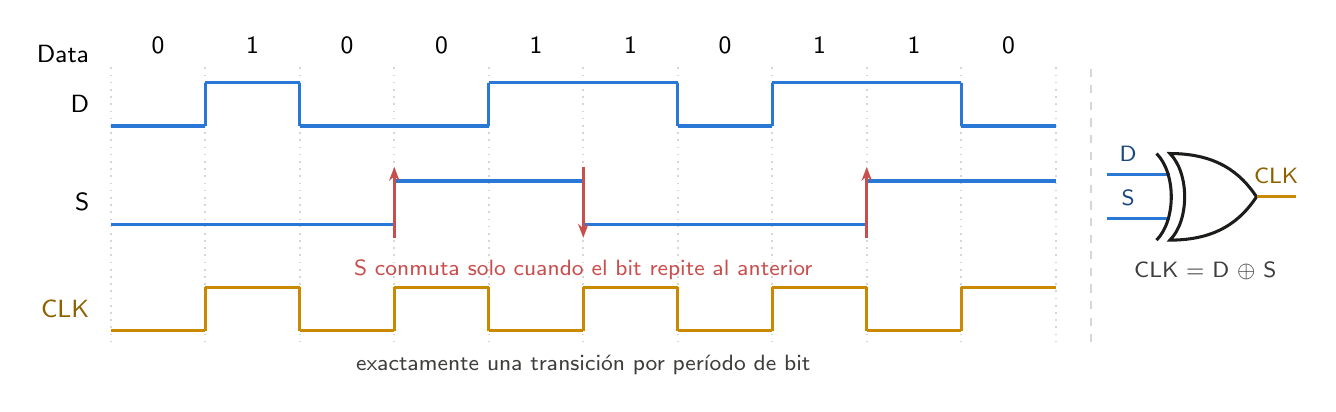
\begin{tikzpicture}[
    x=1cm, y=1cm, font=\sffamily\small,
    rej/.style={draw=cRef!35, dotted, line width=0.6pt},
    wD/.style={draw=cPropio, line width=1.2pt},
    wC/.style={draw=cIP!85!black, line width=1.2pt},
    rot/.style={font=\sffamily\small, anchor=east},
    bit/.style={font=\sffamily\small, anchor=south},
    note/.style={font=\sffamily\footnotesize, text=cRef!45!black},
    sw/.style={-{Stealth[length=5pt]}, draw=cAcc, line width=1.1pt},
]

\def\bw{1.2}     % ancho de un período de bit
\def\amp{0.55}   % excursión de las señales
\def\x{1.5}      % origen del cronograma

% ===================== Rejilla de períodos de bit =====================
\foreach \k in {0,...,10} {\draw[rej] ({\x+\k*\bw},1.05) -- ({\x+\k*\bw},4.55);}

% ===================== Fila de bits =====================
\node[rot] at (1.35,4.72) {Data};
\foreach \b [count=\i from 0] in {0,1,0,0,1,1,0,1,1,0} {
    \node[bit] at ({\x+\i*\bw+0.5*\bw},4.60) {\b};
}

% ===================== Línea Data =====================
\node[rot] at (1.35,4.08) {D};
\foreach \b [count=\i from 0, remember=\b as \lb (initially 0)] in {0,1,0,0,1,1,0,1,1,0} {
    \draw[wD] ({\x+\i*\bw},{3.80+\b*\amp}) -- ({\x+(\i+1)*\bw},{3.80+\b*\amp});
    \draw[wD] ({\x+\i*\bw},{3.80+\lb*\amp}) -- ({\x+\i*\bw},{3.80+\b*\amp});
}

% ===================== Línea Strobe =====================
\node[rot] at (1.35,2.83) {S};
\foreach \b [count=\i from 0, remember=\b as \lb (initially 0)] in {0,0,0,1,1,0,0,0,1,1} {
    \draw[wD] ({\x+\i*\bw},{2.55+\b*\amp}) -- ({\x+(\i+1)*\bw},{2.55+\b*\amp});
    \draw[wD] ({\x+\i*\bw},{2.55+\lb*\amp}) -- ({\x+\i*\bw},{2.55+\b*\amp});
}

% Las tres conmutaciones de Strobe: los bits que repiten al anterior.
\draw[sw] ({\x+3*\bw},2.38) -- ({\x+3*\bw},3.28);
\draw[sw] ({\x+5*\bw},3.28) -- ({\x+5*\bw},2.38);
\draw[sw] ({\x+8*\bw},2.38) -- ({\x+8*\bw},3.28);
\node[note, text=cAcc, anchor=north] at ({\x+5*\bw},2.22)
      {S conmuta solo cuando el bit repite al anterior};

% ===================== Reloj recuperado =====================
\node[rot, text=cIP!60!black] at (1.35,1.48) {CLK};
\foreach \b [count=\i from 0, remember=\b as \lb (initially 0)] in {0,1,0,1,0,1,0,1,0,1} {
    \draw[wC] ({\x+\i*\bw},{1.20+\b*\amp}) -- ({\x+(\i+1)*\bw},{1.20+\b*\amp});
    \draw[wC] ({\x+\i*\bw},{1.20+\lb*\amp}) -- ({\x+\i*\bw},{1.20+\b*\amp});
}
\node[note, anchor=north] at ({\x+5*\bw},1.02)
      {exactamente una transición por período de bit};

% ===================== Puerta XOR: recuperación del reloj =====================
\draw[rej, dashed] (13.95,1.05) -- (13.95,4.55);

\draw[draw=cPropio, line width=1.1pt] (14.15,3.18) -- (14.95,3.18);
\draw[draw=cPropio, line width=1.1pt] (14.15,2.62) -- (14.95,2.62);
\node[note, text=cPropio!60!black, anchor=south] at (14.42,3.22) {D};
\node[note, text=cPropio!60!black, anchor=south] at (14.42,2.66) {S};

% Cuerpo de la puerta, con el arco trasero doble propio de la XOR.
\draw[draw=cRef!20!black, line width=1.1pt, fill=white]
      (14.95,2.35) .. controls (15.20,2.60) and (15.20,3.20) .. (14.95,3.45)
      .. controls (15.55,3.45) and (15.85,3.20) .. (16.05,2.90)
      .. controls (15.85,2.60) and (15.55,2.35) .. (14.95,2.35) -- cycle;
\draw[draw=cRef!20!black, line width=1.1pt]
      (14.78,2.35) .. controls (15.03,2.60) and (15.03,3.20) .. (14.78,3.45);

\draw[draw=cIP!85!black, line width=1.1pt] (16.05,2.90) -- (16.55,2.90);
\node[note, text=cIP!60!black, anchor=south] at (16.30,2.94) {CLK};

\node[note, anchor=north] at (15.40,2.20) {CLK $=$ D $\oplus$ S};

\end{tikzpicture}
\end{document}
